\documentclass[10pt]{article}
\usepackage{icmlko}

\icmlmeta{IP 파운데이션 월드모델}{75}{일흔다섯 건은 아무것도 판정하지 못한다}{애니의 '방향 문제'는 배선을 안 고른 문제였고, 팝업이 옳은지 물었더니 표본이 대답을 못 했다}

\begin{document}

\twocolumn[
\icmlheader

\begin{abstract}
노트 69가 애니메이션의 축이 반대를 가리킨다고 했고 노트 70--73이 그것을 고치는
데 라벨이 얼마나 드는지 쟀다. \textbf{전제가 틀렸다.} 애니는 여덟 도메인 중
\emph{배선 탐색을 한 번도 안 한 유일한 도메인}이었다 --- 웹툰 배선을 그대로
베꼈다. 앙상블 자로 후보를 돌리니 타깃 폭이 태그 수에서 \textbf{연령 등급}으로,
굿즈 규모는 \textbf{끄기}로 간다($\Delta+$0.0680, 씨앗 넷 전부 채택). 애니
앙상블이 $-$0.258에서 \textbf{$+$0.277}로 뒤집히고, 판정치가 $+$0.3235에서
\textbf{$+$0.3915}로, 셀 평균이 $+$0.2291에서 \textbf{$+$0.3615}로 오른다.
그리고 노트 74의 법칙이 \textbf{여덟 도메인 전부에서} 성립한다 --- 자기 $\rho$와
대상 전이의 상관이 $+$0.401에서 \textbf{$+$0.987}로. \textbf{방향 문제라는 것은
없었다.} 후반부는 다른 질문이다 --- 여덟 대상 평균이 팝업의 대리인가. 설정
스물여덟 개에서 $\Delta$판정치와 $\Delta$팝업의 상관이 $+$0.314이고 39\%가
반대 방향이라 ``대리가 아니다''로 보였다. \textbf{짝지은 구간을 붙이니 답이
달랐다} --- $\Delta$팝업의 구간이 전부 0을 포함하고 반폭이 판정치의
\textbf{네 배 이상}이다. 즉 낮은 상관은 판정치가 틀려서가 아니라 \textbf{팝업이 못 재서}다.
판정치와 같은 해상도를 가지려면 팝업 레코드가 \textbf{약 1,650건}, 0.02짜리
효과만 가리려 해도 \textbf{약 510건}이 필요하다. 지금은 75건이다.
\end{abstract}
]

\begin{figure*}[t]
\centering
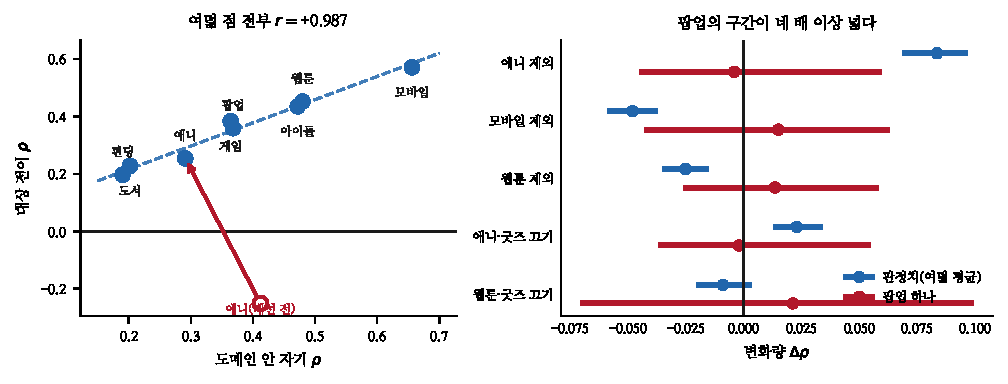
\includegraphics[width=\textwidth]{figs/s75.pdf}
\caption{왼쪽 --- 자기 $\rho$와 대상 전이(빈 표식이 배선 전 애니).
오른쪽 --- 다섯 설정에서 판정치와 팝업의 짝지은 구간.}
\end{figure*}

\section{방향 문제라는 것은 없었다}

애니를 넣을 때 웹툰 배선을 그대로 베꼈다. 웹툰에서 태그 수가 연령 등급을
이겼으므로(노트 46) 같은 자리에 태그 수를 놓았다. \textbf{배선 탐색을 안 했다}
--- 게임 · 도서 · 웹툰 · 펀딩은 전부 후보 열을 돌려 골랐는데 애니만 안 돌렸다.

\begin{table}[t]
\centering\tsize
\caption{애니 배선 후보. 앙상블 자, 여덟 도메인.}
\begin{tabular}{lrr}
\toprule
& 앙상블 & $\Delta$ \\
\midrule
현행(태그 수 · 시리즈 순번) & $+$0.3235 & --- \\
\textbf{타깃 폭 $\leftarrow$ 연령 등급} & $+$0.3547 & \textbf{$+$0.0312} \\
굿즈 규모 끄기 & $+$0.3402 & $+$0.0167 \\
굿즈 규모 $\leftarrow$ 태그 수 & $+$0.3300 & $+$0.0065 \\
타깃 폭 끄기 & $+$0.3285 & $+$0.0050 \\
타깃 폭 $\leftarrow$ 장르 수 & $+$0.3105 & $-$0.0130 \\
굿즈 규모 $\leftarrow$ 화수 & $+$0.3104 & $-$0.0131 \\
타깃 폭 $\leftarrow$ 연령 등급(역) & $+$0.3057 & $-$0.0178 \\
\bottomrule
\end{tabular}
\end{table}

\begin{table}[t]
\centering\tsize
\caption{채택 검정. 씨앗 넷(노트 72 규약), 붓스트랩 150회.}
\begin{tabular}{lrl}
\toprule
& $\Delta$ & 95\% 구간 \\
\midrule
연령 등급 & $+$0.0312 & $[+0.0135, +0.0485]$ 외 3, 전부 채택 \\
\textbf{$+$ 굿즈 끄기} & \textbf{$+$0.0680} & $[+0.0586, +0.0877]$ 외 3, 전부 채택 \\
\bottomrule
\end{tabular}
\end{table}

\paragraph{부호가 반대인 이유를 밝혀 둔다}
다른 여섯에서 타깃 폭은 ``몇 명에게 닿게 만들었나''이고 연령 등급이 높을수록
좁아진다. 애니는 반대다 --- 라프텔은 \emph{유료 애니 구독 서비스}라 주 이용자가
성인이고, 전체 이용가는 아동 대상이라 한줄평을 쓰는 층과 멀다. \textbf{닿는
폭을 일반 인구가 아니라 플랫폼 인구 기준으로 재면 부호가 뒤집힌다.}

굿즈 규모는 껐다. 시리즈 순번이 ``무엇을 얻나''가 아니라 ``얼마나 늦었나''라는
것은 노트 69가 이미 짚었고, 화수로 바꿔도 나빠진다. \textbf{대응물이 없으면
끄는 것이 규약이다.}

\section{법칙이 여덟 점 전부에서 성립한다}

\begin{table}[t]
\centering\tsize
\caption{배선 전후.}
\begin{tabular}{lrr}
\toprule
& 전 & 후 \\
\midrule
앙상블 판정치 & $+$0.3235 & \textbf{$+$0.3915} \\
셀 평균 & $+$0.2291 & \textbf{$+$0.3615} \\
애니 앙상블 & $-$0.258 & \textbf{$+$0.277} \\
자기 $\rho$ vs 대상 & $+$0.401 & \textbf{$+$0.987} \\
자기 $\rho$ vs 출처 & $-$0.182 & $-$0.492 \\
\bottomrule
\end{tabular}
\end{table}

노트 74는 법칙을 보이려고 애니를 빼야 했다($r{=}+0.998$, 일곱 점). 이제
\textbf{여덟 점 전부로 $+$0.987}이다.

\claimx{노트 69--73이 ``방향 문제''라 부른 것은 배선을 안 고른 것이었다.
배선 탐색 후보에 양극성을 다 넣으면 배선 탐색이 곧 부호 결정이고, 나머지 일곱
도메인은 그 과정에서 부호가 이미 정해져 있었다.}{그렇다면 노트 70의 ``방향에
라벨 32건''도 배선 탐색으로 대체할 수 있다는 뜻인데, 확인 안 했다. 배선 탐색은
대상 라벨을 쓰므로 새 카테고리에는 그대로 못 쓴다.}

\section{판정치는 팝업의 대리인가}

노트 72 · 74에서 판정치가 오를 때 팝업이 두 번 내렸다. 설정 스물여덟 개를
만들어 둘을 함께 쟀다 --- 도메인 하나씩 빼기 일곱, 축 하나씩 끄기 스물하나.

\begin{table}[t]
\centering\tsize
\caption{판정치를 가장 많이 올리는 설정 넷.}
\begin{tabular}{lrr}
\toprule
& $\Delta$판정치 & $\Delta$팝업 \\
\midrule
애니 제외 & $+$0.0841 & $-$0.0165 \\
애니·굿즈 끄기 & $+$0.0167 & $-$0.0109 \\
도서 제외 & $+$0.0147 & $-$0.0037 \\
펀딩 제외 & $+$0.0080 & $-$0.0151 \\
\midrule
\multicolumn{2}{l}{상관 $r$ (설정 28개)} & $+$0.314 \\
\multicolumn{2}{l}{방향이 반대인 설정} & 11개 (39\%) \\
\bottomrule
\end{tabular}
\end{table}

넷 다 판정치를 올리고 팝업을 내린다. 여기까지 보면 ``판정치는 팝업의 대리가
아니다''로 읽힌다. \textbf{구간을 붙이기 전까지는 그렇다.}

\begin{table}[t]
\centering\tsize
\caption{짝지은 붓스트랩 150회. 구간 반폭만 적는다 --- 전체 구간은 그림 1.}
\begin{tabular}{lrrr}
\toprule
설정 & 판정치 & 팝업 & 배수 \\
\midrule
애니 제외 & 0.014 & 0.052 & 3.8 \\
모바일 제외 & 0.011 & 0.053 & 4.8 \\
웹툰 제외 & 0.010 & 0.042 & 4.2 \\
애니·굿즈 끄기 & 0.011 & 0.046 & 4.4 \\
웹툰·굿즈 끄기 & 0.012 & 0.085 & 7.0 \\
\midrule
중앙값 & \textbf{0.011} & \textbf{0.052} & \textbf{4.4} \\
\bottomrule
\end{tabular}
\end{table}

\textbf{$\Delta$팝업의 구간이 다섯 개 전부 0을 포함하고} 반폭이 판정치의
\textbf{네 배 이상}이다. 낮은 상관 $+$0.314는 판정치가 틀렸다는 증거가 아니라
\textbf{팝업이 못 잰다는 증거}다.

\noindent\textbf{필요한 표본을 계산한다.}
반폭은 $n^{-1/2}$로 줄어든다. 판정치와 같은 해상도(0.011)를 가지려면
$(0.052/0.011)^2\approx22$배 --- \textbf{약 1,650건}이다. 0.02짜리 효과만
가리려 해도 $(0.052/0.02)^2\approx6.8$배로 \textbf{약 510건}이다. 지금은
75건이고, 이것은 이 루프 밖의 자산이다.

\claimx{팝업 75건으로는 어떤 설계 결정도 팝업 기준으로 판정할 수 없다. 짝지은
$\Delta$팝업의 반폭이 0.052이고, 여기서 재는 결정들의 크기는 0.01--0.08이다.
판정치와 팝업이 갈리는지 여부 자체를 지금 표본으로는 알 수 없다.}{반대로
``갈리지 않는다''는 것도 못 보인다. 두 가능성 다 열려 있다.}

\section{한계}

\begin{itemize}[leftmargin=1.1em,itemsep=0.15em]
\item 애니 배선을 앙상블 자로 골랐는데, 그 자를 정한 것도 이 프로젝트다.
      다른 자였으면 다른 배선을 골랐을 것이다.
\item ``연령 등급 부호가 반대인 이유''는 사후 해석이다. 채택 근거는 검정이다.
\item 애니가 굿즈 규모를 잃어 공통 축이 둘이 됐고, 게임(매장 축이 꺼져 있다)과는
      공통 축이 하나뿐이라 \textbf{두 셀이 사라졌다}(56$\to$54). 판정치 상승의
      일부가 그 두 셀이 빠진 것일 수 있다.
\item 팝업 필요 표본 계산이 $n^{-1/2}$ 가정에 기댄다. 노트 68이 그 가정이 깨지는
      경우를 봤다.
\item 대리 실험의 설정 스물여덟 개는 전부 ``빼기''다. ``더하기'' 설정은 안 봤다.
\end{itemize}

\section{다음}

\begin{enumerate}[leftmargin=1.3em,itemsep=0.15em]
\item 사라진 두 셀(게임$\leftrightarrow$애니)을 살린다 --- 게임 매장 축을 켜거나
      애니 굿즈 대응물을 찾는다.
\item 나머지 일곱 도메인의 배선을 앙상블 자로 다시 돌린다. 애니 하나에서
      $+$0.068이 나왔다면 다른 데도 있을 것이다.
\item 아홉째 도메인 --- 셀 54$\to$72.
\item 팝업 표본. 510건이 되기 전에는 팝업 기준 판정을 포기하고 판정치를 따른다.
\end{enumerate}

\vspace{0.6em}
\hrule height 0.3pt
\vspace{0.5em}
{\footnotesize
\textbf{참고문헌}\\[0.3em]
Spearman, C. (1904). The proof and measurement of association between two things.
\emph{American Journal of Psychology}, 15(1), 72--101.\\[0.15em]
Efron, B., Tibshirani, R. J. (1993). \emph{An Introduction to the Bootstrap}.
Chapman \& Hall.\\[0.15em]
Kish, L. (1965). \emph{Survey Sampling}. Wiley.\\[0.15em]
Cawley, G. C., Talbot, N. L. C. (2010). On over-fitting in model selection and
subsequent selection bias in performance evaluation. \emph{JMLR}, 11, 2079--2107.\\[0.15em]
Ben-David, S. et al. (2010). A theory of learning from different domains.
\emph{Machine Learning}, 79(1--2), 151--175.
}

\end{document}
